\section{Auftrieb und Strömungswiderstand}

Dieser Versuch soll die Funktionsweise einer Tragfläche demonstrieren und auch den Einfluss des Anstellwinkels auf den Auftrieb (Kraft nach oben) und Rücktrieb aufzeigen. Mit diesen Werten sollen der beste Anstellwinkel der Tragfläche gefunden werden, was durch das Verhältnis von Auftriebs- und Widerstandskraft ausgedrückt wird. Da dieser Term gleichzeitig bei einem Gleitflug das Verhältnis von zurückgelegter Wegstrecke und Höhenverlust darstellt und somit ein guter Indikator für den besten Anstellwinkel der Tragfläche ist.

\subsection{Messaufbau}

Die Tragfläche wird an einer Auftriebswaage befestig, wobei gleichzeitig durch einen Kraftmesser der Rücktrieb gemessen werden kann. Dann wird mit einer konstante Windgeschwindigkeit von \SI{14.38}{\metre\per\second} und für verschieden Anstellwinkel der Tragfläche der Auftrieb und der Rücktrieb gemessen.

\subsection{Auswertung}

\begin{figure}
    \centering
    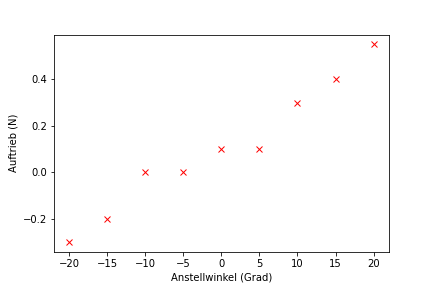
\includegraphics[scale=0.8]{Aeromechanik/Protokoll/fig/Aeromechanik Versuch 3.11.png}
    \caption{Verhältnis von Auftrieb und Anstellwinkel bei konstanter Windgeschwindigkeit}
    \label{fig:Aeoromechanik Versuch 3.11}
\end{figure}

\begin{figure}
    \centering
    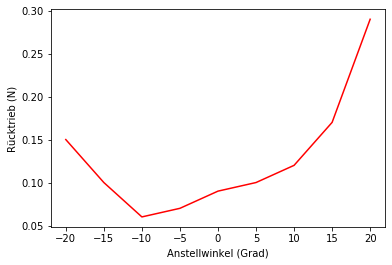
\includegraphics[scale=0.8]{Aeromechanik/Protokoll/fig/Aeromechanik Versuch 3.12.png}
    \caption{Verhältnis von Rücktrieb und Anstellwinkel bei konstanter Windgeschwindigkeit}
    \label{fig:Aeromechanik Versuch 3.12}
\end{figure}

\begin{figure}
    \centering
    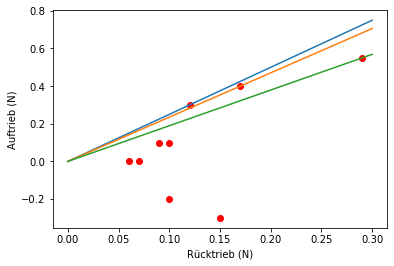
\includegraphics[scale=0.8]{Aeromechanik/Protokoll/fig/Aeromechanik Versuch 3.13.png}
    \caption{Verhältnis von Auftrieb und Rücktrieb bei konstanter Windgeschwindigkeit um die größte Gleitzahl zu finden}
    \label{fig:Aeromechanik Versuch 3.13}
\end{figure}

\section{Druckmessung}
\subsection{Messaufbau}